% =============================================================================
% appendix_h_teacher.tex -- Appendix H, additional teacher results. Owner: Results writer. New 12 Nov 2026.
% Holds the details of the teacher analysis that the condensed Section 5.7 (06_results.tex) no longer carries and
% that are not already in Appendix F (05_diagnostics.tex) or Appendix D (appendix_d_figures.tex). Text from the
% draft of 8 Nov (commit ae2c88b, 06_results.tex lines 202-441), condensed in wording only.
% Run identifiers: the teacher = Final, uncorrected teacher = Control, initial model = Base, teacher with full /
% partial shape mask = Final-masked / Final-partial-mask (Table~\ref{tab:names}).
% =============================================================================

\chapter{Additional teacher results}
\label{app:teacher-extra}

This appendix collects observations and open points of the teacher analysis (Section~\ref{sec:res-teacher-ablations})
that are not needed for its findings. All statements refer to single runs on the sets of
Section~\ref{sec:res-setup}.

\section{Holdout examples and reconstruction}

\begin{figure}[!b]
\centering\small
\setlength{\tabcolsep}{0pt}
\begin{tabular}{@{}*{4}{>{\centering\arraybackslash}p{0.25\linewidth}}@{}}
Image & Ground truth & Initial model & Teacher \\
\end{tabular}\\[2pt]
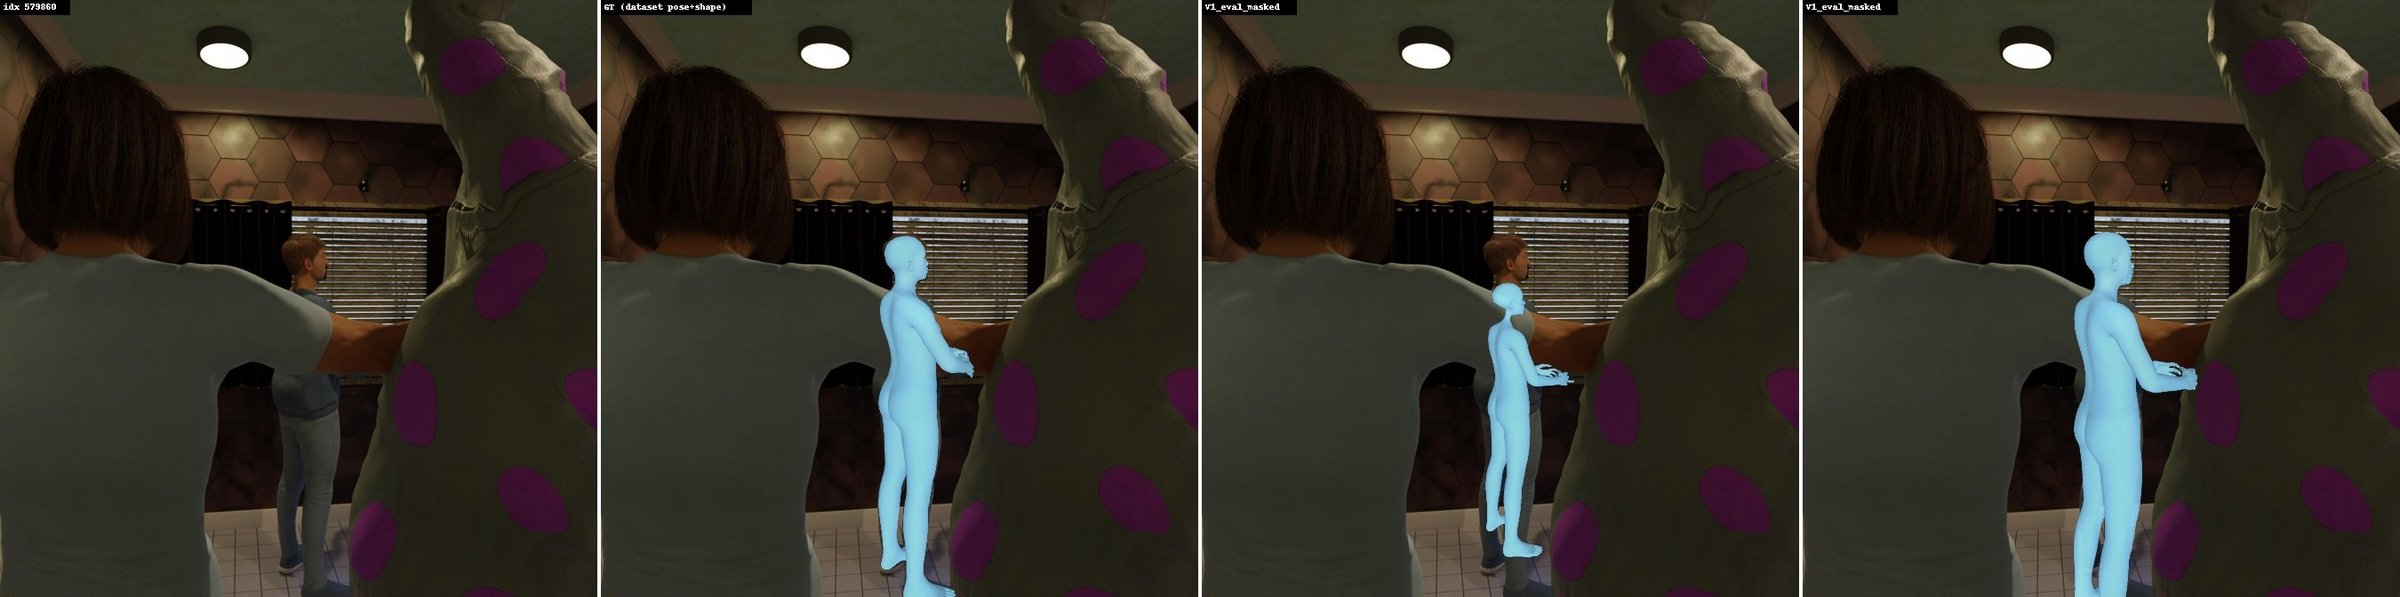
\includegraphics[width=\linewidth, trim=0 0 0 16, clip]{F12_holdout_579860_img_gt_base_final}\\[4pt]
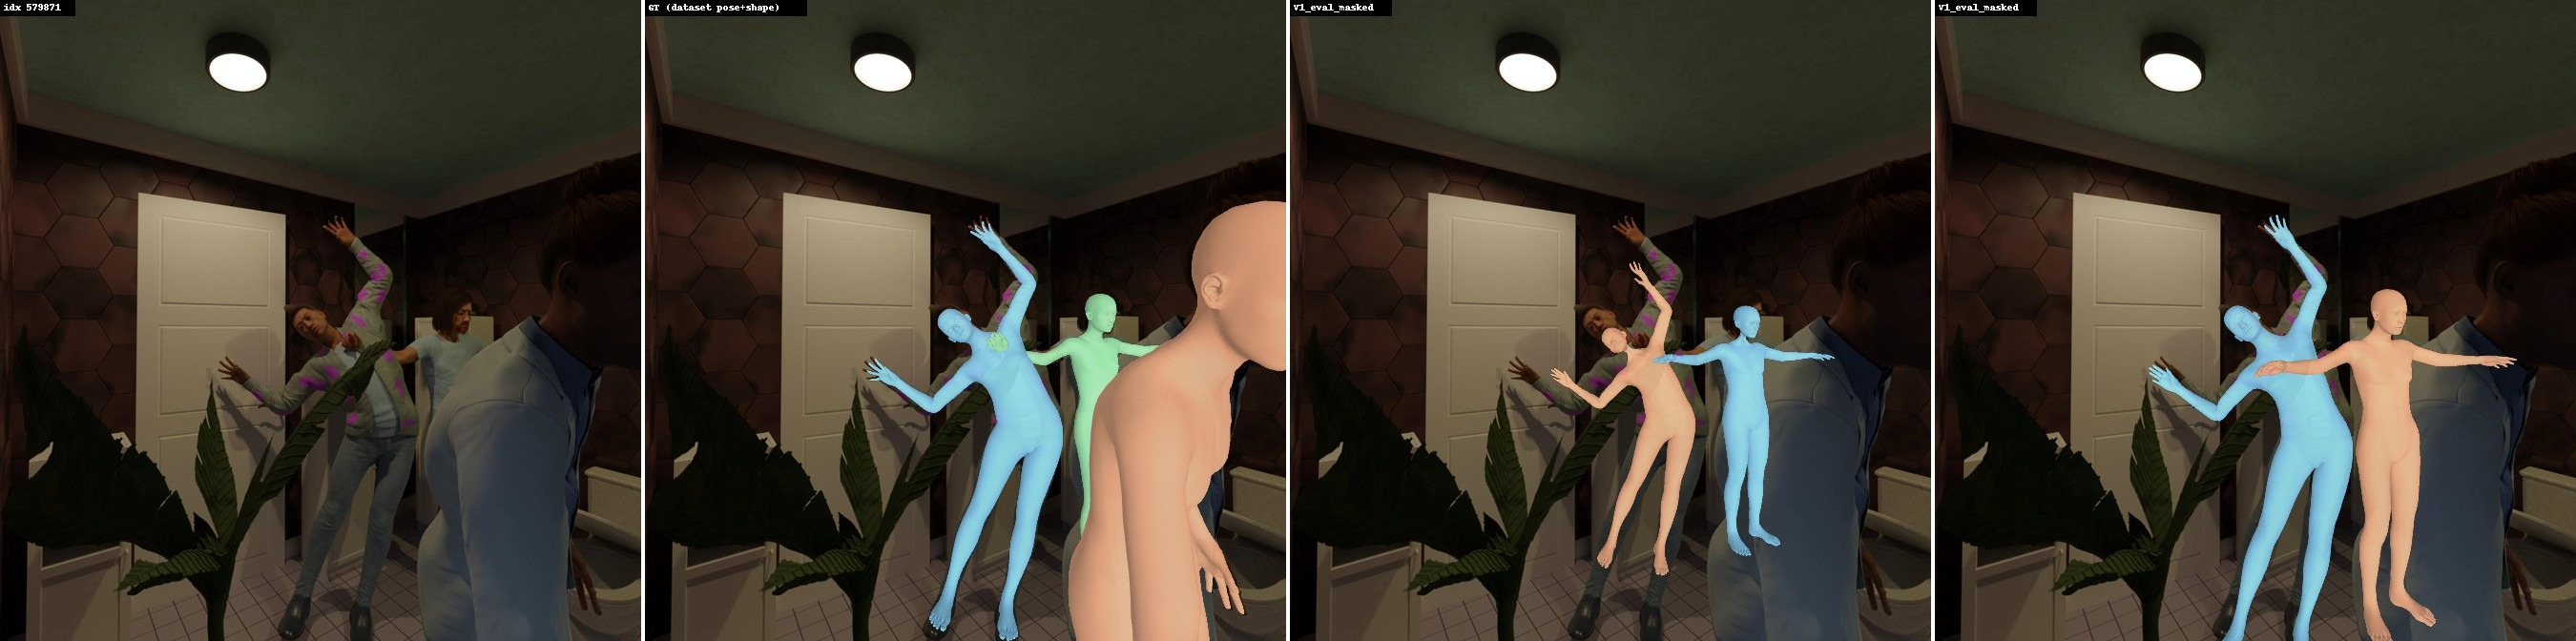
\includegraphics[width=\linewidth, trim=0 0 0 16, clip]{F12_holdout_579871_img_gt_base_final}
\caption[Two further holdout images]{Two further AnnyOne holdout images (579860 top, 579871 bottom), arranged as in
Figure~\ref{fig:holdout-montage}. The ground truth is drawn with the dataset camera, the predictions of the initial
model (Base) and the teacher (Final) with the holdout protocol, each body at its model's predicted depth.}
\label{fig:holdout-montage-more}
\end{figure}

Figure~\ref{fig:holdout-montage-more} shows the two holdout images of the earlier four-image figure that are not
repeated in Section~\ref{sec:res-final}; in the original renderings the prediction panels carry the label
``V1\_eval\_masked''. In all four images mesh colours mark detections, not identities; people without a
ground-truth mesh (the foreground arm in 579862) are not scored, and people a model misses (the two lying in the
foreground of 579865) have no mesh. During training the teacher stayed below the uncorrected teacher at all ten
epochs on 3DPW validation, whereas on the holdout the two alternated (Figure~\ref{fig:val-curves}).

The comparison of the teacher with the uncorrected teacher has four gaps. The matched sets differ in size
(\FinalMatched, \ControlMatched{} and \BaseMatched{} people) and PVE was not compared on the same people, recall was
not computed separately for people with a visible head (which would test the explanation via the moved detection
cell), no bootstrap intervals were computed, and there is no second run of the teacher.

On the 3DPW overlays (Figure~\ref{fig:3dpw-overlays}) most men receive male bodies from the teacher and
female-looking ones from the initial model, the teacher's bodies are slightly larger, and the seated guitar player is
reconstructed poorly by both. The low 3DPW precision arises because every detected bystander and every ghost body on
a half-visible person counts as a false positive. The run-to-run variation on 3DPW was not measured. The 3DPW result was not broken down by sequence, and only 8 frames were inspected
visually.

\section{Placement}

The teacher's pelvis lands farther from its true pixel than the uncorrected teacher's (\FinalPelvisPx{} against
\ControlPelvisPx{} pixels), probably because the head is pinned while the body is still drawn too small. Its root
error is also above that of the depth pilot (\num{\DepthPilotRootErr}\,mm), possibly because of the real images or
the bone correction. Neither explanation was tested, and the reason why the slope of predicted against true depth
does not move is unknown. The single-image figure of the depth fix (Figure~\ref{fig:depth-579862}), in which the initial model draws the
man far behind his true position and too small and the depth pilot close to his true size, shows the depth pilot,
not the teacher.

\section{Bone correction}

On the real frame of Figure~\ref{fig:neck-3dpw-bar}, which no model trained on, the initial model draws both
necks as thin stalks under the head and the corrected model draws them at normal width. The frame shows the neck
pilot, not the teacher, and its columns also differ
by the fine-tune. On the holdout, however, the same fine-tune without the correction keeps the girth at
\BaseGirth{} (Table~\ref{tab:neck-bones}), so the correction is the likely cause of the wider necks. Flips that
cancel each other along a chain (Section~\ref{sec:diag-neck}) would need a two-sided correction, which was not
implemented.

\section{Fingers on real images}

In the crops of Figure~\ref{fig:fingers-demo}, which are the first demos with predicted instead of rest-pose
fingers, the initial model's fingers are splayed and stiff, and one finger of the left hand sticks out as the
flipped metacarpal1.L would make it. The teacher's hands lie over the armrest in the party photo, are curled as if
fretting in the guitar frame, and bend over the edge of the bar in the bar frame. Small hands
(Figure~\ref{fig:fingers-all}) cannot be judged at print size.

\section{Body shape}

On the demo photos (Figures~\ref{fig:real-photos} and~\ref{fig:photo-montages}) most men look male with the teacher,
and the boy keeps an adult body. The gender gain is consistent with the corrected 3DPW gender labels, which supervise
the shape head on real people for the first time. Only detected people are scored on Relative Human, so the matched
sets differ between models.

At the cut-off 0.5 the gender accuracy of the two masked models is near chance only because both sexes moved up, so
most men are classified as women. A cut-off for real photos would have to be chosen on 3DPW validation, which was not
done; the best accuracy in Table~\ref{tab:gender-auc} uses a cut-off chosen on Relative Human itself and therefore
only shows the size of the threshold effect. On the AnnyOne holdout only \HoldGenderLabelAboveHalf\,\% of the gender
labels lie above 0.5. The partial mask restores weight spread on real photos, but not muscle spread.

In the rest-pose line-up (Figure~\ref{fig:rest-lineup}) only the body differs. The initial model gives nearly
everyone the same slim, flat body. The teacher gives the singers a fuller chest and hips and the man in the bar a
broader torso. The tennis players stay slim in all three models, in line with the intermediate gender score of men,
and the teacher with full shape mask resembles the teacher except for a slimmer man in the bar. The explanation of
the weakened muscle correlation by the converter's constant muscle value of \MethodConstOther{} was not tested.

\section{Shape-supervision masking}

The 3DPW mesh targets still hold the neutral body under both masks, which is why the body errors barely change. With
age supervised (partial mask) the age-group improvement remains in this run; this suggests an effect of the age
target but does not establish the mechanism. Gender accuracy falls under both masks although the gender label stays
supervised. One untested reading is that the teacher's gender gain depends on the seven constants on the 3DPW men as
much as on the gender label. The partial-mask model had no demo run, so it is not known whether it restores variety on
the demo images, and the reason why gender falls remains open.
